%%% LaTeX Template: Two column article
%%%
%%% Source: http://www.howtotex.com/
%%% Feel free to distribute this template, but please keep to referal to http://www.howtotex.com/ here.
%%% Date: February 2011

%%% Preamble
\documentclass[	DIV=calc,%
							paper=a4,%
							fontsize=12pt,%
							onecolumn]{scrartcl}	 					% KOMA-article class

\usepackage{lipsum}													% Package to create dummy text
\usepackage[brazil]{babel}										% English language/hyphenation
\usepackage[protrusion=true,expansion=true]{microtype}				% Better typography
\usepackage{amsmath,amsfonts,amsthm}					% Math packages
\usepackage[pdftex]{graphicx}									% Enable pdflatex
\usepackage[svgnames]{xcolor}									% Enabling colors by their 'svgnames'
\usepackage[hang, small,labelfont=bf,up,textfont=it,up]{caption}	% Custom captions under/above floats
\usepackage{epstopdf}												% Converts .eps to .pdf
\usepackage{subfig}													% Subfigures
\usepackage{booktabs}												% Nicer tables
\usepackage{fix-cm}													% Custom fontsizes
\usepackage[utf8]{inputenc}
\usepackage[top=2.5cm, bottom=2.5cm, left=2.5cm, right=2.5cm]{geometry}
\usepackage[ddmmyyyy]{datetime}
\addto\captionsenglish{%
	\renewcommand\tablename{Tabela}
	\renewcommand\figurename{Figura}
} 
 

 
%%% Custom sectioning (sectsty package)
\usepackage{sectsty}													% Custom sectioning (see below)
\allsectionsfont{%															% Change font of al section commands
	\usefont{OT1}{phv}{b}{n}%										% bch-b-n: CharterBT-Bold font
	}

\sectionfont{%																% Change font of \section command
	\usefont{OT1}{phv}{b}{n}%										% bch-b-n: CharterBT-Bold font
	}



%%% Headers and footers
\usepackage{fancyhdr}												% Needed to define custom headers/footers
	\pagestyle{fancy}														% Enabling the custom headers/footers
\usepackage{lastpage}	

% Header (empty)
\lhead{}
\chead{}
\rhead{}
% Footer (you may change this to your own needs)

%% ====================================
%% ====================================
%% mude o rodape  do projeto
%% ====================================
%% ====================================

\lfoot{\footnotesize \texttt{Cabeamento estruturado} \textbullet ~Projeto}


\cfoot{}
\rfoot{\footnotesize página \thepage\ de \pageref{LastPage}}	% "Page 1 of 2"
\renewcommand{\headrulewidth}{0.0pt}
\renewcommand{\footrulewidth}{0.4pt}



%%% Creating an initial of the very first character of the content
\usepackage{lettrine}
\newcommand{\initial}[1]{%
     \lettrine[lines=3,lhang=0.3,nindent=0em]{
     				\color{DarkGoldenrod}
     				{\textsf{#1}}}{}}



%%% Title, author and date metadata
\usepackage{titling}															% For custom titles

\newcommand{\HorRule}{\color{DarkGoldenrod}%			% Creating a horizontal rule
									  	\rule{\linewidth}{1pt}%
										}

\pretitle{\vspace{-30pt} \begin{flushleft} \HorRule 
				\fontsize{50}{50} \usefont{OT1}{phv}{b}{n} \color{DarkRed} \selectfont 
				}

%% ====================================
%% ====================================
%% mude o titulo  do projeto
%% ====================================
%% ====================================

\title{Projeto de cabeamento estruturado}					% Title of your article goes here

%% ====================================



\posttitle{\par\end{flushleft}\vskip 0.5em}

\preauthor{\begin{flushleft}
					\large \lineskip 0.5em \usefont{OT1}{phv}{b}{sl} \color{DarkRed}}
\author{Heitor Poso Polizeli,Eduardo José Silvestre}  	% Author name goes here


\postauthor{\footnotesize \usefont{OT1}{phv}{m}{sl} \color{Black} 
					\\Universidade Tecnológica Federal do Paraná - Câmpus Cornélio Procópio 								% Institution of author
					\par\end{flushleft}\HorRule}

\date{}																				% No date




%%% Begin document
\begin{document}
\maketitle
\thispagestyle{fancy} 	
\thispagestyle{empty}		% Enabling the custom headers/footers for the first page 
% The first character should be within \initial{}




%% ====================================
%% ====================================
%% mude o resumo  do projeto
%% ====================================
%% ====================================
\initial{E}\textbf{Esta documentação tem como objetivo demonstrar na prática a elaboração de um projeto
	de cabeamento estruturado, embasando-se em normas nacionais e internacionais como,
	por exemplo, NBR-14565-2007 e TIA/EIA-568-B. A implantação do presente projeto será realizado de forma fictícia em um edifício comercial de dois andares, onde o piso 1 possui 6 salas e o piso 2 possui 10 salas com tomadas de telecomunicações.A rede de cabeamento estruturado sera criada do zero com o intuito de administrar de uma forma precisa e eficaz os recursos de dados e voz, atendendo as necessidades momentâneas e futuras de uma organização. Os elementos de rede presente nos pisos serão devidamente identificados utilizando-se de padrões, o layout se da por meio de um cabeamento horizontal que interliga cada area de trabalho aos armários de telecomunicações presentes nos dois pisos e esses por sua vez são interligados por um backbone.     }

%% ====================================
\begin{figure}
	\centering
	\includegraphics{utfpr}
\end{figure}

\vspace{3cm}
\centerline{\textit{\textbf{\today}}}

\clearpage
    \renewcommand*\listfigurename{Lista de figuras}
\listoffigures

\renewcommand*\listtablename{Lista de tabelas}
\listoftables




\clearpage
\renewcommand{\contentsname}{Sumário}
\tableofcontents
\clearpage

%% ====================================
%% ====================================
%% Inicio do texto
%% ====================================
%% ====================================
\section{Introdução}
  O projeto tem a finalidade de atender a necessidade de interligação de dois andares, sendo
  o piso 1 com 6 salas e o piso 2 com 10 salas, levando pontos de redes com acesso a dados e
  voz, por meio de cabeamento horizontal para cada área de trabalho do edifício. Atualmente
  o prédio  não conta com nenhum equipamento de TI facilitando a implantação do projeto
  em questão. Basicamente o projeto utilizaria um armário de telecomunicação em cada piso interligados por um backbone e em cada armário de telecomunicação teremos um path panel e switch para dados e um path panel e switch para voz. 
  
\subsection{Benefícios}

Com a implantação de um projeto de cabeamento estruturado seguindo normas como
NBR-14565-2007 e TIA/EIA-568-B os principais benefícios são:

 • Probabilidade de ocorrer erros na camada física é menor por conta dos equipamentos
e testes realizados no processo;

 • A identificação de problemas posteriores na camada física podem ser localizados de
forma mais fácil por conta da identificação dos pontos de redes;

 • Uma rede estruturada esta preparada para um processo de ampliação.



\subsection{Usuários}

A estrutura contará inicialmente com 16 tomadas de telecomunicação distribuídas nas
salas do piso 1, onde as salas 1 e 4 terão 4 tomadas cada uma e as demais salas terão 2
tomadas cada. O piso 2 contará com 23 tomadas de telecomunicação sendo que a sala
2 possuirá 3 tomadas e a sala 3 possuirá 4 tomadas, as demais sala do piso terão duas
tomadas de telecomunicação cada uma. A maioria das salas possuem 2 tomadas pois
para o processo de certificação essa é a quantidade mínima de pontos para cada área de
trabalho, porém a estrutura final contará com a possibilidade de ampliação da rede como
um todo, visto que a empresa possui metas de crescimento e o projeto   de cabeamento
estruturado visa atender essa expansão.



\section{Estrutura predial existente}

A estrutura a ser atendida com o projeto de cabeamento estruturado é composta por 2
pisos. O piso 1 possui 250m2, dividido em 6 salas e o piso 2,250m2,divido em 10 salas,
sendo que ambos possuem estrutura para passagem do cabeamento, como eletrocalhas,
canaletas, dutos e caixas de passagem. 


\section{Planta Lógica - Elementos estruturados}


\subsection{Topologia}

No piso 1 foi inserido um armário de telecomunicações, que contem dois Path Panels
de 24 portas, e esses estão diretamente conectados a dois Switches de 24 portas. Esses
equipamentos estão divididos da seguinte maneira um Switch e um Path Panel disponível
para dados e um Switch e um Path Panel disponível para voz e uma régua de energia, todos
esses equipamentos estão localizados em um rack de 24U 670mm, disponibilizando um
total de 32 pontos de comunicação, dividindo-se em dezesseis para dados e dezesseis para
voz, interconectando as seis salas presentes nesse piso. No piso 2 foi inserido um armário
de telecomunicações, que contem dois Path Panels de 48 portas, e esses estão diretamente
conectados a dois Switches de 48 portas. Esses equipamentos estão divididos da seguinte
maneira um Switch e um Path Panel disponível para dados e um Switch e um Path Panel
disponível para voz e uma régua de energia, todos esses equipamentos estão localizados
em um rack de 24U 670mm, disponibilizando um total de 46 pontos de comunicação,
dividindo-se em vinte e três para dados e vinte e três para voz, interconectando as dez salas
presentes nesse piso. A interligação dos pavimentos utiliza-se de um backbone composto
de fibra optica 2 pares. A Figura 1 ilustra o layout dessa topologia acima descrita e a
Figura 2 é a legenda dos equipamentos apresentados na Figura 1.





\begin{figure}
	\centering
	\includegraphics[width=0.7\linewidth]{diagramalogicorede}
	\caption{Diagrama Lógico de Rede }
	\label{fig:diagramalogicorede}
\end{figure}
\subsection{Encaminhamento}

	
O cabeamento foi realizado em dois pisos de um edifício comercial, utilizando-se de
eletrocalhas embutidas na parede, as tomadas de telecomunicações que disponibilizam
dados e voz estão a 45 cm do chão conforme as normas de cabeamento estruturado.
\subsection{Memorial descritivo}

Na Figura 3 temos os principais equipamentos que serão utilizados para a elaboração do
projeto com a estimativa de quantidade, abaixo da tabela segue as especificações dos equipamentos de maior relevância 

\begin{figure}
	\centering
	\includegraphics[width=0.7\linewidth]{legendaequip}
	\caption{ Legenda Dos Equipamentos }
	\label{fig:legendaequip}
\end{figure}

\begin{figure}
	\centering
	\includegraphics[width=0.7\linewidth]{quant_equip}
	\caption{Quantidade Dos Equipamentos }
	\label{fig:quantequip}
\end{figure}

Na Figura 4 apresenta o Armário de telecomunicação utilizado no piso 1 e 2, com as seguintes especificações : 

* Material: A¸co

* Espessura: 2,00 mm

* Espessura Portas e Laterais: 1,20 mm

* Altura: 2100 mm

* Largura: 600 mm

* Profundidade: 800mm

* Peso: 112Kg


\begin{figure}
	\centering
	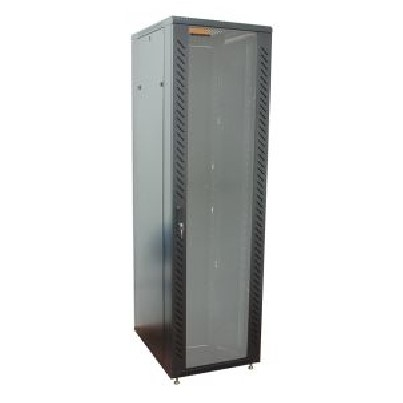
\includegraphics[width=0.7\linewidth]{racktelecom}
	\caption{ Armário de Telecomunicação}
	\label{fig:racktelecom}
\end{figure}


Figura 5 apresenta Switch de 48 portas utilizado no piso 2 para atender as 10 salas
presentes no andar. O Cisco Catalyst 3550 12G, empilhavel, fornecem alta disponibilidade, segurança e qualidade de serviço (QoS) para melhorar o funcionamento da rede. 


\begin{figure}
	\centering
	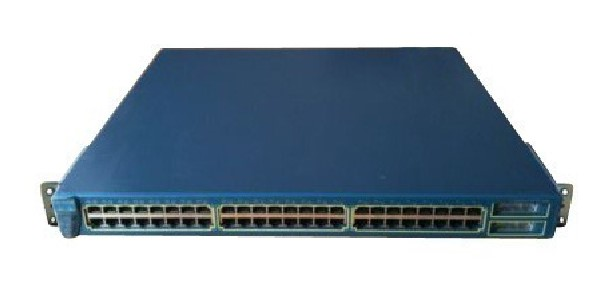
\includegraphics[width=0.7\linewidth]{switch}
	\caption{Switch Cisco }
	\label{fig:switch}
\end{figure}


Figura 6 apresenta Switch de 24 portas utilizado no piso 1 para atender as 6 salas
presentes no andar. Switch com Configuração Fixa 24 portas Gigabit 10/100/1000
que suportam conexões de alto desempenho. Priorização IEEE 802.1p que oferece compatibilidade com as redes que suportam aplicações de tempo real. Pode ser montado em armários ou empilhado para otimizar o espaço, sua altura de 1U padrão simplifica o planejamento do espaço.
\begin{figure}
	\centering
	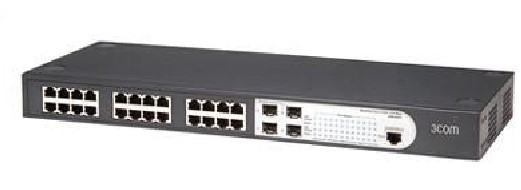
\includegraphics[width=0.7\linewidth]{switchm}
	\caption{Switch Gigabit /10/100/1000}
	\label{fig:switchm}
\end{figure}

Figura 7 apresenta Path Panel de 24 e 48 portas utilizados nos armários de telecomunicação que interliga o cabeamento horizontal aos Switches.

• Excede os requisitos estabelecidos nas normas para CAT.6 / Classe E

• Performance garantida para até 6 conexões em canais de até 100 metros

• 24 ou 48 posições RJ-45

• Painel frontal em plastico com porta etiquetas para identificação. 

• Possui borda de reforço para evitar empenamento

• Fornecido com parafusos e arruelas para fixar 

• Fornecido com ícones de identificação o e velcros para organiza¸c˜ao


\begin{figure}
	\centering
	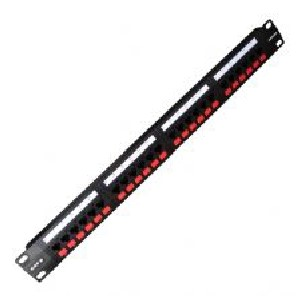
\includegraphics[width=0.7\linewidth]{pathcpanel}
	\caption{Patch Panel }
	\label{fig:pathcpanel}
\end{figure}

Figura 8 apresenta a régua utilizado nos armários de telecomunicação com a seguinte
característica 

• Régua sem disjuntor com 8 tomadas para Armários de telecomunicação e cabo com 1,5 mts


\begin{figure}
	\centering
	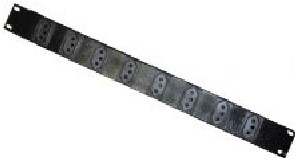
\includegraphics[width=0.7\linewidth]{reguaene}
	\caption{Régua Alimentação}
	\label{fig:reguaene}
\end{figure}

\subsection{Identificação dos cabos}
A tabela 4 representa a identificação dos pontos das 6 salas presentes no piso 1. A tabela
5 representa a identificação dos pontos das 10 salas presentes no piso 2, com a seguinte
legenda:

*  TO -  Numero da tomada de telecomunicação 

*  A -   Dados

*  B -   Voz

*  SL -  Sala

*  P -   Piso.

\section{Implantação}
Estabeleça um cronograma de implantação:
Remoção de equipamentos existentes (destino para descarte), instalação dos condutores, instalação dos cabos, 
identificação dos cabos, montagem dos racks, certificação, etc... Crie atividades e estabeleça o tempo de execução. Se for um projeto real, indique também quais os responsáveis pela execução do projeto e de cada uma das etapas.

Defina marcas (e padrões) e fornecedores se for o caso. Atenção a contratados e subcontratados para a realização das atividades. Estabeleça a responsabilidade de execução da atividade e também da validação dela.

Utilize algum software para gerear o cronograma. Excel,etc. O fundamental é dividir em etapas, descrever e estimar o tempo de cada uma delas.

Segue uma relação de ferramentas:
http://asana.com/, 
https://trello.com/, 
http://www.ganttproject.biz/, 
http://www.orangescrum.org/. 

\section{Plano de certificação}
Quais seriam as etapas para a certificação? 
Quais os locais e horários para execução da certificação na rede? Toda rede será certificada?
Como os testes seriam executados?
Quais relatórios de certificação serão (ou deveriam ser) entregues? 

\section{Plano de manutenção}

Revisões periódicas na rede, emissão de certificados para novos pontos.

\subsection{Plano de expansão}
Existe um plano de expansão? Quantos novos pontos poderão ser acrecidos na rede, antes de migração de equipamentos na camada 2? Se houver expansão, quais equipamentos deverão ser direcionados para as estremidades da rede? 

\section{Risco}
Se tratando de um projeto estruturado e bem projetado, não corremos nenhum risco. 

\section{Orçamento}
Crie uma relação de orçamentos baseado na seções anteriores.


\section{Referências bibliográficas}
Utilize o mendley, o jabref ou diretamente o bibtex para gerenciar suas referências biliográficas. As referências são criadas automaticamente de acordo com o uso no texto.

Exemplo: Redes de computadores, segundo \cite{t2013} é considerada..... Já \cite{kurose2010} apresenta uma versão...

Analisando os pressupostos de \cite{ref3} e \cite{ref4} concluimos que....


\renewcommand\refname{} %%Referências bibliográficas}  
\bibliographystyle{ieeetr}
\bibliography{referencias}  

%% ***********************************************************************
%% === remover daqui =====================================================
%% ***********************************************************************
=================================================
\section{Elementos textuais - Alguns exemplos}

Esta seção apresenta exemplos de elementos textuais. \textbf{Remova-a da versão final do texto}.


\subsection{Colocar elementos em itens}

Texto antes da lista

\begin{itemize}
	\item First item in a list 
	\item Second item in a list 
	\item Third item in a list
\end{itemize}

\subsubsection{Uma subseção de terceiro nivel}

Exemplo de uma subseção

\subsection{Tabelas}

Utilize o site http://www.tablesgenerator.com/ para elaborar as tabelas de seu trabalho.
Para adicionar uma tabela utilize: a tag input, passando o arquivo da tabela como parametro

\input{tab2}

Dentro do arquivo você deve definir o label e pode utilizá-lo para referenciar. Exemplo:
Na tab \ref{tab2} temos a relação de ....


Você também pode modificar a tabela manualmente, incluindo, por exemplo h! dentro de sua definição. Veja no exemplo tab2.tex



%% ***********************************************************************
%% === ate aqui    =====  ================================================
%% ***********************************************************************

\end{document}